%
% teil2.tex -- Beispiel-File für teil2 
%
% (c) 2020 Prof Dr Andreas Müller, Hochschule Rapperswil
%
% !TEX root = ../../buch.tex
% !TEX encoding = UTF-8
%
\section{Analyse der Daten 
\label{milankovic:section:WissenschaftlicheArbeit}}

\subsection{Motivation
	\label{milankovic:subsection:Motivation}}
In den bisherigen Kapiteln ist die Bedeutung der Milankovic-Zyklen deutlich geworden. Als Bestandteil der weiteren Arbeit werden die Milankovic-Zyklen auf selbstständiger Basis rekonstruiert und mit den Werten aus der Literatur verlichen. So werden die Daten unabhängig überprüft und allfällige Diskrepanzen aufgezeigt. Ausserdem steigt das Verständnis für die Zusammenhänge der einzelnen Parameter mit den Auswirkungen auf das ganze System. 

\subsection{Vorgehen
\label{milankovic:subsection:Vorgehen}}
Mit einfachen Mitteln erfolgt die Untersuchung der online abrufbaren Daten.
Der Bezug erfolgt vom IMCCE, dem Institut für Himmelsmechanik und Ephemeriedenberechnung in Paris.
\cite{milankovic:vo.imcce.fr}
Unter den Datensätzen, die bis 250 Millionen Jahre zurückreichen, galt es sich auf einen Zeitraum von rund 5 Millionen Jahre zu beschränken, da so die Übersichtlichkeit und auch die Darstellbarkeit der Ergebnisse, bei ausreichender Genauigkeit, gewährleistet werden kann.
Die Auswahl ist dabei auf den Zeitraum von 6 bis 2 Millionen Jahre vor heute gefallen.
Es sind marginale Unterschiede feststellbar, wenn die folgenden Untersuchungen für andere oder längere Zeiträume geführt werden.

\subsection{Untersuchung
\label{milankovic:subsection:Untersuchung}}
Aus den Daten sind die absoluten Werte der einzelnen Zyklen ablesbar.
In der Darstellung mit Microsoft-Excel wird ein harmonischer Verlauf sichtbar.
Mit der Untersuchung der Fast Fourier Transformation (FFT) werden die Häufigkeiten der massgebenden Frequenzen ermittelt.
Um die FFT-Untersuchung durchführen zu können ist das Add-In Analyse-Funktionen zu installieren.
Damit die Darstellung gelingt, kann in Excel direkt von der Darstellung in der komplexen Schreibweise auf die normale gewechselt werden.
Nach der Umrechnung der Abszissenachse in besser lesbare Dimensionen, treten je nach untersuchtem Zyklus verschieden scharfe Peaks auf, die mit den Angaben der Milankovic-Zyklen übereinstimmen.
So kann davon ausgegangen werden, dass sich die Zyklen tatsächlich in diesen Grössenordnungen bewegen.
Einige Ausschläge sind etwas schärfer als andere.
Diese Unschärfe wird auch bei der Bestimmung der Periodizitäten ersichtlich, denn einige Angaben schwanken im Bereich um wenige Jahrtausende.
Bei der Untersuchung verschiedener Perioden kann festgestellt werden, dass gewisse Ausschläge geringen Schwankungen unterliegen.

Bei der Betrachtung der Analyse der Exzentrizität
(Abbildung \ref{pictureUntersuchungExzentrizität})
ist ersichtlich, dass im Bereich von 100ka (Jahrtausend) ein etwas breiterer Peak erkennbar ist, der sich aus einigen kleineren Ausschlägen und einem etwas Deutlicheren zusammensetzt, und bei 400ka der Ausschlag äusserst scharf und prägnant ist.

\begin{figure}
	\centering
	\includegraphics[width=\linewidth]{papers/milankovic/pictures/02_Exzentrizität.pdf}
	\caption{Untersuchung Exzentrizität
		\label{pictureUntersuchungExzentrizität}}
\end{figure}

Die Frequenzen der Erdachsneigung sind deutlich durch einen Peak um 41ka beeinflusst.
	(Abbildung \ref{pictureUntersuchungObliquität})
Kleinere Ausschläge sind im Bereich von rund 60ka und 30ka erkennbar, die eine untergeordnete Rolle spielen und nicht an die Intensität des Hauptausschlages herankommen.

\begin{figure}
	\centering
	\includegraphics[width=\linewidth]{papers/milankovic/pictures/03_Obliquität.pdf}
	\caption{Untersuchung Obliquität
		\label{pictureUntersuchungObliquität}}
\end{figure}

Bei der Präzession
\ref{pictureUntersuchungPräzession}
ist neben den Peaks um 23ka ein verstärktes Rauschen erkennbar.
Dies kann unter anderem auf Unsicherheiten in der Berechnung, ausgelöst durch die Kontinentalverschiebung, zurückgeführt werden.
Die beiden Peaks bei 23ka bestätigen, dass die in anderen Dokumenten auftretenden Frequenzen zwischen 20ka und 26ka durchaus ihre Berechtigung haben.
Besonders bei der Präzession sind verschiedene Angaben bezüglich der Periodizität verbreitet.


\begin{figure}
	\centering
	\includegraphics[width=\linewidth]{papers/milankovic/pictures/04_Präzession.pdf}
	\caption{Untersuchung Präzession
		\label{pictureUntersuchungPräzession}}
\end{figure}

\subsection{Einwirkungen auf das Klima
\label{milankovic:subsection:EinwirkungenKlima}}
Unter Berücksichtigung aller Milankovic-Zyklen lässt sich die Veränderung der Sonneneinstrahlungsintensität auf die Erdoberfläche berechnen.
(Abbildung \ref{pictureUntersuchungSonneneinstrahlungsintensität})
Dadurch wird der Wärmeeintrag auf die Erde und somit auch auf die Atmosphäre beschrieben. Standardmässig wird dies für den 65igsten nördlichen Breitengrad gemacht.
Dies entspricht ungefähr dem Rand der grösstmöglichen Eisschilde in Eiszeiten.
Bei der Untersuchung des Intensitätverlaufes mit FFT sind die beiden Frequenzen von Obliquität und Präzession deutlich erkennbar, was auf eine Abhängigkeit schliessen lässt.
Um die berechneten Werte zu überprüfen, ist ein Abgleich mit der Realität anzustreben.

Mit der Untersuchung von Bohrkernen, die an den Polen entnommen wurden, kann der geschichtliche Temperaturverlauf rekonstruiert werden.
Dort wird der Niederschlag für unbestimmte Zeit in den Gletschern konserviert. Über das Verhältnis von stabilen Sauerstoffatomen, der sogenannten Sauerstoffisotopenmethode (Delta O18-Methode), ist dabei die Temperaturveränderung zwischen zeitlichen Perioden bestimmbar.
Wird dieser Verlauf auch mit FFT untersucht, treten Ausschläge auf, die mit den Frequenzen der Milankovic-Zyklen korrespondieren.
(Abbildung \ref{pictureUntersuchungKonzentration})
Die Daten zeigen einen zeitlich klaren Kausalzusammenhang.

\begin{figure}
	\centering
	\includegraphics[width=\linewidth]{papers/milankovic/pictures/05_Sonneneinstrahlungsintensität.pdf}
	\caption{Untersuchung Sonneneinstrahlungsintensität
		\label{pictureUntersuchungSonneneinstrahlungsintensität}}
\end{figure}
\begin{figure}
	\centering
	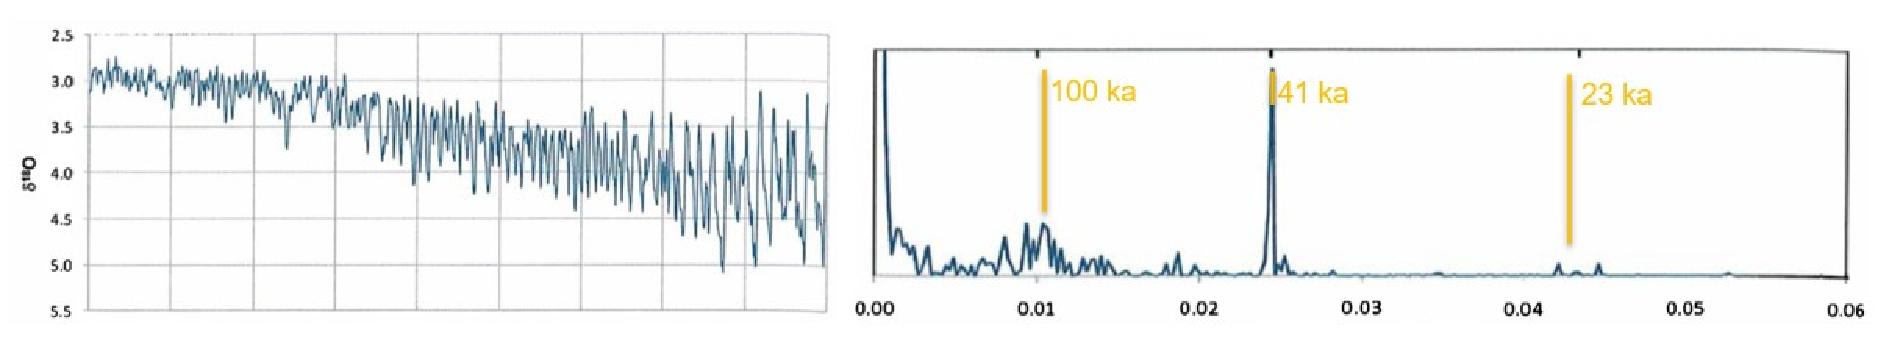
\includegraphics[width=\linewidth]{papers/milankovic/pictures/06_O18-Konzentration.pdf}
	\caption{Untersuchung Sauerstoffisotopgehalt mittles O18-Methode
		\label{pictureUntersuchungKonzentration}}
\end{figure}

\subsection{Folgen für das Klima
	\label{milankovic:subsection:FolgenKlima}}
Da wir die Milankovic-Zyklen berechnen können und diese das Klima direkt beeinflussen, sollte die Berechnung der klimatischen Veränderungen ebenfalls mögliche sein.
Grundsätzlich ist dies, wie eingangs beschrieben, der Fall, denn infolge der Zyklen steuert die Erde auf eine gemässigte Glazialperiode zu.
Jedoch ist festzuhalten, dass das Klima durch viele weitere Effekte beeinflusst wird.
Die klimatischen Bedingungen ausschliesslich den Zyklen zuzuordnen wäre falsch.
Es ist ein äusserst komplexes Thema rund um die Bildung des Klimas.
Viele Phänomene wirken sich auf das Klima aus.
Einen besonders starken Effekt erzielt dabei der Eintrag von Treibhausgasen und Aerosolen in die Atmosphäre, ungeachtet dessen, ob der Ursprung bei der Natur oder dem Menschen liegt.

Einen direkten Vergleich zwischen den Milankovic-Zyklen und dem Einfluss des Menschen auf das Klima ist kaum möglich, denn die Messperioden und Messunsicherheiten sind schlecht miteinander vergleichbar.
Im Bereich der Erdbewegung wird in Jahrtausenden gerechnet, wo der wesentliche Einfluss des Menschen auf die Atmosphäre einige Jahrzehnte alt ist.
Auch die Unsicherheiten betrachtend fällt ein Vergleich schwer.
Zwischen absoluten aktuellen Werten mit noch nie zuvor erreichter Präzision und Jahrtausende gelagertem Gletschereis, das bei deren Bildung unterschiedlichen Einflüssen ausgesetzt war besteht eine grosse Diskrepanz in der Hinsicht auf die Unsicherheit bei der Festlegung der Temperatur.

jl



